\documentclass[tikz]{standalone}

%% Language and font encodings
\usepackage[english]{babel}
\usepackage[utf8x]{inputenc}
\usepackage[T1]{fontenc}

\usepackage{xcolor}
\definecolor{darkblue}{HTML}{1f4e79}
\definecolor{lightblue}{HTML}{00b0f0}
\definecolor{salmon}{HTML}{ff9c6b}
\definecolor{purple}{HTML}{9933ff}

\usetikzlibrary{backgrounds,calc,shadings,shapes.arrows,arrows,shapes.symbols,shadows,positioning,decorations.markings,backgrounds,arrows.meta}

% Define parallelepiped shape:
\makeatletter
\pgfkeys{/pgf/.cd,
  parallelepiped offset x/.initial=2mm,
  parallelepiped offset y/.initial=2mm
}
\pgfdeclareshape{parallelepiped}
{
  \inheritsavedanchors[from=rectangle]
  \inheritanchorborder[from=rectangle]
  \inheritanchor[from=rectangle]{north}
  \inheritanchor[from=rectangle]{north west}
  \inheritanchor[from=rectangle]{north east}
  \inheritanchor[from=rectangle]{center}
  \inheritanchor[from=rectangle]{west}
  \inheritanchor[from=rectangle]{east}
  \inheritanchor[from=rectangle]{mid}
  \inheritanchor[from=rectangle]{mid west}
  \inheritanchor[from=rectangle]{mid east}
  \inheritanchor[from=rectangle]{base}
  \inheritanchor[from=rectangle]{base west}
  \inheritanchor[from=rectangle]{base east}
  \inheritanchor[from=rectangle]{south}
  \inheritanchor[from=rectangle]{south west}
  \inheritanchor[from=rectangle]{south east}
  \backgroundpath{
    \southwest \pgf@xa=\pgf@x \pgf@ya=\pgf@y
    \northeast \pgf@xb=\pgf@x \pgf@yb=\pgf@y
    \pgfmathsetlength\pgfutil@tempdima{\pgfkeysvalueof{/pgf/parallelepiped offset x}}
    \pgfmathsetlength\pgfutil@tempdimb{\pgfkeysvalueof{/pgf/parallelepiped offset y}}
    \def\ppd@offset{\pgfpoint{\pgfutil@tempdima}{\pgfutil@tempdimb}}
    \pgfpathmoveto{\pgfqpoint{\pgf@xa}{\pgf@ya}}
    \pgfpathlineto{\pgfqpoint{\pgf@xb}{\pgf@ya}}
    \pgfpathlineto{\pgfqpoint{\pgf@xb}{\pgf@yb}}
    \pgfpathlineto{\pgfqpoint{\pgf@xa}{\pgf@yb}}
    \pgfpathclose
    \pgfpathmoveto{\pgfqpoint{\pgf@xb}{\pgf@ya}}
    \pgfpathlineto{\pgfpointadd{\pgfpoint{\pgf@xb}{\pgf@ya}}{\ppd@offset}}
    \pgfpathlineto{\pgfpointadd{\pgfpoint{\pgf@xb}{\pgf@yb}}{\ppd@offset}}
    \pgfpathlineto{\pgfpointadd{\pgfpoint{\pgf@xa}{\pgf@yb}}{\ppd@offset}}
    \pgfpathlineto{\pgfqpoint{\pgf@xa}{\pgf@yb}}
    \pgfpathmoveto{\pgfqpoint{\pgf@xb}{\pgf@yb}}
    \pgfpathlineto{\pgfpointadd{\pgfpoint{\pgf@xb}{\pgf@yb}}{\ppd@offset}}
  }
}
\makeatother

\tikzset{
  dense/.style={
    parallelepiped,fill=white, draw,
    minimum width=0.8cm,
    minimum height=1.2cm,
    parallelepiped offset x=0.3cm,
    parallelepiped offset y=0.3cm,
    path picture={
      \draw[top color=darkblue,bottom color=darkblue]
        (path picture bounding box.south west) rectangle 
        (path picture bounding box.north east);
    },
    text=white,
  },
  fourier/.style={
    parallelepiped,fill=white, draw,
    minimum width=1.2cm,
    minimum height=2.4cm,
    parallelepiped offset x=0.5cm,
    parallelepiped offset y=0.5cm,
    path picture={
      \draw[top color=salmon,bottom color=salmon]
        (path picture bounding box.south west) rectangle 
        (path picture bounding box.north east);
    },
    text=white,
  },
  linear/.style={
    parallelepiped,fill=white, draw,
    minimum width=1.2cm,
    minimum height=2.4cm,
    parallelepiped offset x=0.5cm,
    parallelepiped offset y=0.5cm,
    path picture={
      \draw[top color=purple,bottom color=purple]
        (path picture bounding box.south west) rectangle 
        (path picture bounding box.north east);
    },
    text=white,
  },
  link/.style={
    color=black,
    line width=0.5mm,
    ->,
  },
}

\begin{document}

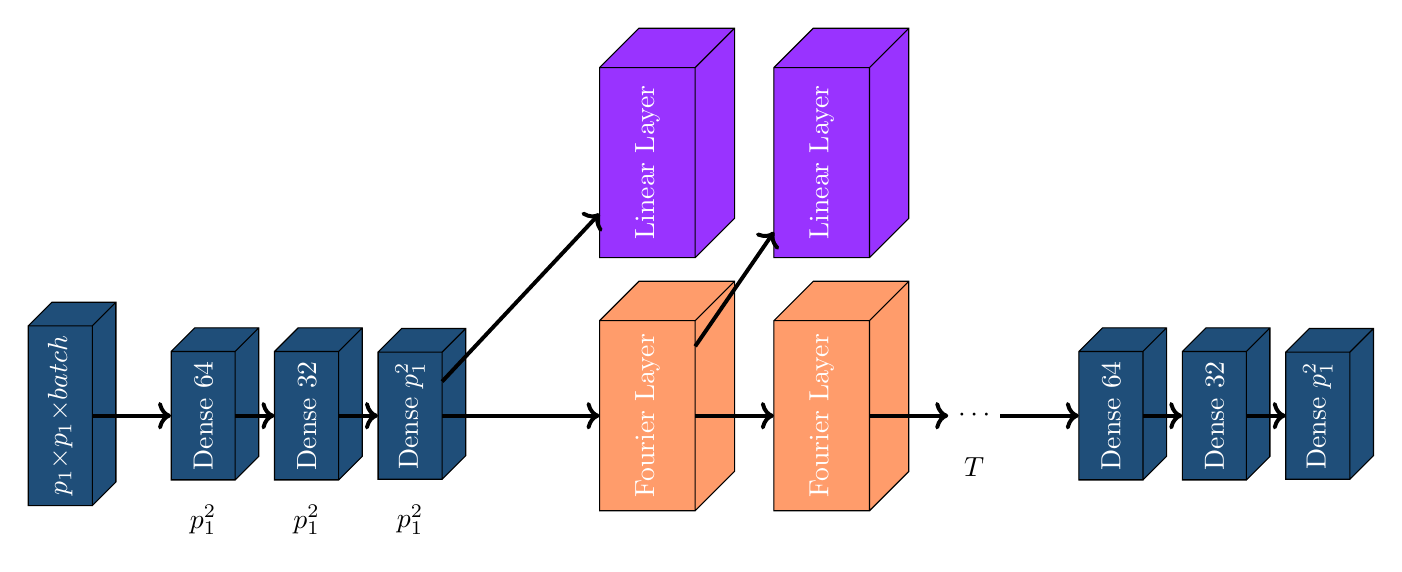
\begin{tikzpicture}
  % Input shape
  \node[dense](input){\rotatebox{90}{$p_1{\times}p_1{\times}batch$}};

  % First Dense Network (64->32->p1*p1)
  \node[dense,right=1cm of input](dense1){\rotatebox{90}{Dense 64}};
  \node[below=0.2cm of dense1]{\rotatebox{0}{$p_1^2$}};
  
  \node[dense,right=0.5cm of dense1](dense2){\rotatebox{90}{Dense 32}};
  \node[below=0.2cm of dense2]{\rotatebox{0}{$p_1^2$}};
  
  \node[dense,right=0.5cm of dense2](dense3){\rotatebox{90}{Dense $p_1^2$}};
  \node[below=0.2cm of dense3]{\rotatebox{0}{$p_1^2$}};

  % First Fourier Network (2 layers)
  \node[fourier,right=2cm of dense3](fourier1){\rotatebox{90}{Fourier Layer}};
  \node[linear,above=0.8cm of fourier1](linear1){\rotatebox{90}{Linear Layer}};
  
  \node[fourier,right=1cm of fourier1](fourier2){\rotatebox{90}{Fourier Layer}};
  \node[linear,above=0.8cm of fourier2](linear2){\rotatebox{90}{Linear Layer}};

  % Dots indicating more layers
  \node[right=1cm of fourier2](dots){$\cdots$};
  \node[below=0.2cm of dots]{$T$};

  % Last Dense Network (64->32->p1*p1)
  \node[dense,right=1cm of dots](dense4){\rotatebox{90}{Dense 64}};
  \node[dense,right=0.5cm of dense4](dense5){\rotatebox{90}{Dense 32}};
  \node[dense,right=0.5cm of dense5](dense6){\rotatebox{90}{Dense $p_1^2$}};

  % Connections
  \draw[->,link] (input) -- (dense1);
  \draw[->,link] (dense1) -- (dense2);
  \draw[->,link] (dense2) -- (dense3);
  \draw[->,link] (dense3) -- (fourier1);
  \draw[->,link] (dense3) -- (linear1);

  \draw[->,link] (fourier1) -- (fourier2);
  \draw[->,link] (fourier1) -- (linear2);
  \draw[->,link] (fourier2) -- (dots);
  
  \draw[->,link] (dots) -- (dense4);
  \draw[->,link] (dense4) -- (dense5);
  \draw[->,link] (dense5) -- (dense6);

\end{tikzpicture}

\end{document}